\begin{figure}[ht]
    \centering
    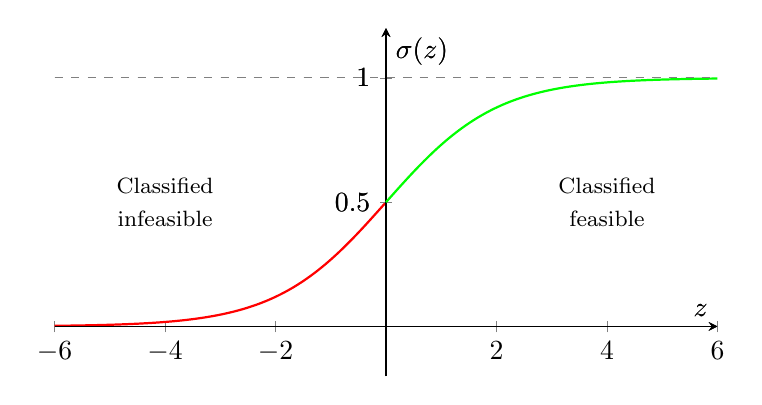
\begin{tikzpicture}
        \begin{axis}[
                axis lines=middle,
                xlabel={$z$},
                ylabel={$\sigma(z)$},
                samples=200,
                domain=-6:0,
                ymin=-0.2, ymax=1.2,
                xtick={-6,-4,-2,0},
                ytick={0,0.5,1},
                width=10cm,
                height=6cm,
            ]
            % Logistic function
            \addplot[red, thick] {1/(1+exp(-x))};

            %Text
            \node[rectangle,minimum width=24pt,align=center] (test)  at (-4,  0.5) {\footnotesize Classified \\ \footnotesize infeasible};

            % Dotted lines for y=0 and y=1
            \addplot[dashed, gray] coordinates {(-6,1) (6,1)};
        \end{axis}
        \begin{axis}[
                axis lines=middle,
                xlabel={$z$},
                ylabel={$\sigma(z)$},
                samples=200,
                domain=0:6,
                ymin=-0.2, ymax=1.2,
                xtick={2,4,6},
                ytick={0,0.5,1},
                width=10cm,
                height=6cm,
            ]
            % Logistic function
            \addplot[green, thick] {1/(1+exp(-x))};

            %Text
            \node[rectangle,minimum width=24pt,align=center] (test)  at (4,  0.5) {\footnotesize Classified \\ \footnotesize feasible};

            % Dotted lines for y=0 and y=1
            \addplot[dashed, gray] coordinates {(-6,1) (6,1)};
        \end{axis}
    \end{tikzpicture}
    \caption{Transformation of linear regression to logistic regression via the sigmoid function.}
    \label{fig:LR_plot}
\end{figure}